% -*- root: root.tex -*-
\RequirePackage[l2tabu, orthodox]{nag}                  % Checks for obsolete syntax and package % Layout
\documentclass[11pt,a4paper,oneside]{article}

%% font
\usepackage{MnSymbol}
\usepackage[mathlf,textlf]{MinionPro}
\usepackage[T1]{fontenc}
\usepackage{enumitem}
\usepackage[utf8]{inputenc}

%% Author
\def\myaffiliation{University of Copenhagen}
\def\myauthor{Rud Faden}
\def\myemail{rud.faden@econ.ku.dk}
\def\mytitle{No cure no pay contracts with limited liability}
\def\mykeywords{Information aggregation, physician,}

%% packages
\usepackage[drafting]{faden}
\pgfplotsset{compat=1.9}
\usetikzlibrary{decorations.pathreplacing}
\graphicspath{{../fig/}}
\usepackage{commath}
\usepackage[colorinlistoftodos,draft]{todonotes}        % todo notes
\setlength{\marginparwidth}{3.5cm} % fix for todo notes


%% custom macroes 

%% biblatex path
\addbibresource{Remote.bib}

% Author and title
\title{\mytitle}
\author{
{\myauthor} \\
\textit{\small \myaffiliation} \\
\small{\texttt{\href{\myemail}{\myemail}}}
}
\date{\today} % no date

%% Version control
\immediate\write18{sh ./vc}
%%% This file has been generated by the vc bundle for TeX.
%%% Do not edit this file!
%%%
%%% Define Git specific macros.
\gdef\GITHash{9d5e3b469d5f4d8f56c54cfc33fcab676c8905ff}%
\gdef\GITAbrHash{9d5e3b4}%
\gdef\GITParentHashes{904e5d3ddc0482da848ff729ca2451b0fd5c4aee}%
\gdef\GITAbrParentHashes{904e5d3}%
\gdef\GITAuthorName{Rud Faden}%
\gdef\GITAuthorEmail{rudfaden@gmail.com}%
\gdef\GITAuthorDate{2015-04-27 11:47:18 +0200}%
\gdef\GITCommitterName{Rud Faden}%
\gdef\GITCommitterEmail{rudfaden@gmail.com}%
\gdef\GITCommitterDate{2015-04-27 11:47:18 +0200}%
%%% Define generic version control macros.
\gdef\VCRevision{\GITAbrHash}%
\gdef\VCAuthor{\GITAuthorName}%
\gdef\VCDateRAW{2015-04-27}%
\gdef\VCDateISO{2015-04-27}%
\gdef\VCDateTEX{2015/04/27}%
\gdef\VCTime{11:47:18 +0200}%
\gdef\VCModifiedText{\textcolor{red}{with local modifications!}}%
%%% Assume clean working copy.
\gdef\VCModified{0}%
\gdef\VCRevisionMod{\VCRevision}%



\begin{document}
\maketitle
\begin{abstract}
This paper examines a pricipal-agent model in which a risk neutral physician makes an ex-ante effort choice. The physician recives payment, only if he cures the patients (e.g. the DRG-value). In the production, the physician employes costly hospital. In his contract with the hospital, the physician is subject to statutory limited liabilty. Given these liability limits, the question is then which contract the hospital optimally offers the physician. 
\end{abstract}
\section{Model} % (fold)
\label{sec:model}
There is a risk neutral physician that cures a continuom of patients with a monetary value of $y\in[0,\infty)$. The physician cures patient with effort $e$. I assume that the probability of curing a patient is monotonically increasing in effort (monotone likelihood ratio property), such that 
\begin{align}
    \pder{y}\left(\frac{g_e(y\mid e)}{g(y\mid e)}\right)>0 \label{eq:mlrp}
\end{align}
for all $e>0$ and $y\ge 0$. In addition I assume that $\cEX{y|e=0}=0$

The principal observes the physicians value of cured patients ex-ante. Therefor the hospital specifies a contract that rquires the physician to repay the hospital as a function of production $R(y)$.

Further it is assumed that the physicians payoff is bounded by limited liability. This implies that (i) the physician cannot be required to pay the hospital more than the value of the production, and (ii) the hospital cannot be required to make payments to the physician.  Therefore the payment function is bounded by $0\leq R(y)\leq y$.

Let $U(y,e)$ denote the physicians continuous and twice differential utility function given by 
\begin{align}
    U(e)=y-R(y)-C(e) \label{eq:utility}
\end{align}.

Given \cref{eq:utility} and a fixed payment function $R(y)$, the physician will choose effort to solve the following problem
\begin{subequations}
\begin{align}
    \max_{y} & \int_0^{\infty}(y-R(y))g(y|e)\dif y-C(e)\label{eq:max-utility} \\
    \text{s.t. }    & \int_{0}^{\infty} R(y)g(y|e)\dif y\geq R_L^0 \label{eq:minimum-payment} \\
                    & \cEX{V(R,e)|e}\leq \cEX{V(R,e^*)|e} \label{eq:optimal-effort}\\
                    & 0\leq R(y)\leq y \label{eq:limited-liability}
\end{align}
\end{subequations}

\begin{proposition}
\label{prop:payment-function}
If $R$ solves the maximization problem in \cref{eq:max-utility}, then there is some threshold value $y^*$, such that 
\[
    R^*(y)=\left\{
    \begin{matrix}
    y               & \text{for } y< y^* \\
    0 & \text{for } y\geq y^*
    \end{matrix} \right.
\]

\end{proposition}

\begin{proof}
Replacing \cref{eq:optimal-effort} with it's first order condtition, and writing down the Lagrangian I get that 
\begin{align}
    \mathcal{L}=\left(y-R(y)\right)\left(g(y|e)+\mu g_e(y|e)\right)-\mu C_e(e)+\lambda R(y)g(y|e)-\lambda C(e)
\end{align}
which can also be written as 
\begin{equation}
\begin{split}
   (\lambda-1)R(y)g(y|e) & -\mu R(y)g_e(y|e)+ \\
                         & y\left(g(y|e)+\mu g_e(y|e)\right)-\mu C_e(e)-\lambda C(e) \label{eq:lagrange}
\end{split}
\end{equation}

Only the first to terms of \cref{eq:lagrange} depends on the size of $R(y)$ and thereby determines the maximum. If the first term is larger than the second term
\begin{align}
    (\lambda-1)g(y|e)\geq \mu f_e(y|e) \label{eq:max-payment}
\end{align}

the whole expression is increasing in $R(y)$, therefore $R(y)$ should be set to it's maximum $R(y)=y$. If the opposite is true 
\begin{align}
    (\lambda-1)g(y|e)< \mu f_e(y|e) \label{eq:min-payment}
\end{align}
the expression is decreasing in $R$, and $R(y)$ should be set to it's minimun $R(y)=0$. Note that \cref{eq:max-payment} can be written as
\begin{align}
    \frac{g_e(y|e)}{g(y|e)}\leq \frac{\lambda-1}{\mu}, \quad \lambda\ne 1,\: \mu\ne 0 \label{eq:min-payment-2}
\end{align}
Given \cref{eq:mlrp}, the left hand side of \cref{eq:min-payment-2} is increasing in $y$ this inequality is satisfied for some $y$ below a threshold level $y^*$. Above $y^*$ \cref{eq:max-payment} holds. Thereby the payment function is 0 for some $y<y^*$ and $y$ for some level above $y\geq y^*$ as stated in \cref{prop:payment-function}
\end{proof}

\begin{figure}[htbp]
    \centering
    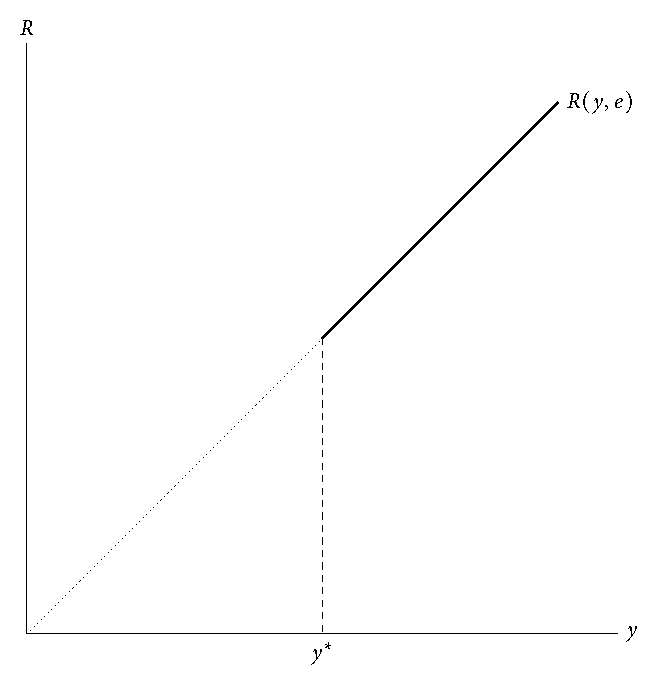
\includegraphics[width=0.95\textwidth]{optimal-R.pdf}
    \caption{The payment function $R(y)$. Before $y^*$ the physician is payed nothing and after $y^*$ the physican is the payed maximum of $R(y)$ }
    \label{fig:label}
\end{figure}


% Unfortunately neither existence or uniqueness and of a solution to \cref{eq:max-utility} can be guaranteed. To reduce the ambiguity I introduce the first assumption 

% \begin{assumption}
% \label{asump:effort}
%  There exists a finite $e_{\max}$ such that 
% \[
%     \lim_{e \rightarrow e_{\max}} \cEX*{U(y,e)|e}<\cEX*{U(y,0)|0}
% \]
%  \end{assumption}

%  \Cref{asump:effort} indicates that there is some disutility to effort and that this effort is increases as $e\rightarrow e_{\max}$. Therefore the physicians effort choice can be limited to $\left[0,e_{\max}\right]$

% \begin{lemma}
% \label{lem:bounded}
% For all $R(y)$ functions satisfying limited liability $0\leq R(y)\leq y$, (i) $\cEX{U(y,e)|e}$ is bounded from above and below on the domain $e\in\left[0,e_{\max}\right]$, and therefore there exists at least one solution to \cref{eq:max-utility}
% \end{lemma} 

% \begin{proof}
% For all $R(y)$ satisfying the limited liability constraint $\cEX{U(y,e)|e}\geq\cEX{U(R(y),e)|e}$, and for $e\in\left[0,e_{\max}\right]$, $\cEX{U(R(y),e)|e}\allowbreak\geq\cEX{U(0,e)|e}\allowbreak\geq\cEX{U(R(y)-k^*,e)|e}$, $k^*=\cEX{R(y)|e_{\max}}$. Since $\cEX{U(R(y),e)|e}$ and thereby also $\cEX{U(R(y)-k^*,e)|e}$ is continuous on the compact set $e\in\left[0,e_{\max}\right]$, implying result (i). Result (ii) then follows from the extreme value theorem.
% \end{proof}

% \Cref{lem:bounded} implies that there exists an optimal level of effort given a eligible payoff function. 
% section model (end)
\end{document}